% !TEX encoding = UTF-8 Unicode
\documentclass[BachelorPaper]{subfiles}
\acresetall
%Providecommands für Subfiles
    \providecommand{\citepic}[1]{(#1)}
    \providecommand{\citefig}[2]{(#1, S. #2)}
    \providecommand{\citefigm}[2]{(Modifiziert #1, S. #2)}

\begin{document}
\chapter{Methods}
The following sections include the steps taken to create the BOINSO network applications and the way the distinct components exchange information.

\section{BOINSO Core Web Application}
\label{sec:methods_boinso_core}

\begin{figure}[!htbp]
\centering
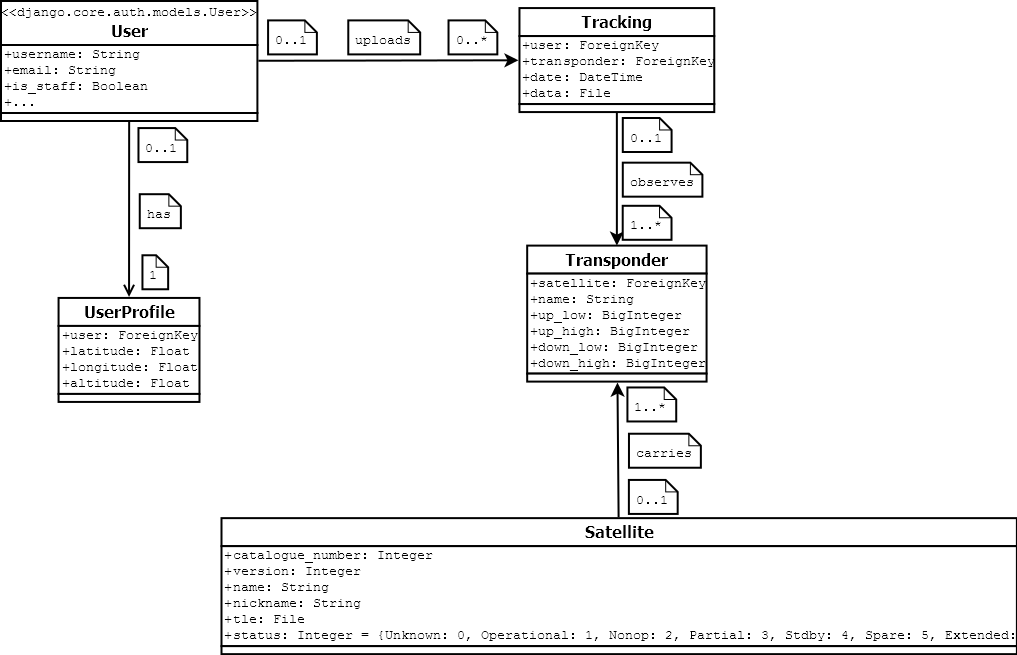
\includegraphics[width=0.9\linewidth]{PICs/diagrams/boinso_core_models.png}
\caption{BOINSO Core Web Application model graph}\label{fig:boinso_core_models}
\end{figure}

As seen in figure \ref{fig:boinso_core_models} the model graph was modeled with only a view important entities as the initial functionality only includes passive satellite passes --  meaning the tracking of a reoccurring transponder transmission.

\end{document}